The system-based and agent-based models use the same seven classes and transitions. Here we present the seven-compartment model as well as the shared assumptions and parameters between the models.%Throughout the three models we utilize the same assumptions and compartment-state definitions. 

\subsection{Compartment-State Definition}
Based on the model and parameters published by Rivers et al.\cite{Rivers2014}, this model divides the population into seven compartments: susceptible (S), exposed (E), infected (I), recovered (R), hospitalized (H), funeralized (F), and dead (D) individuals. The permissible transitions are as pictured in Figure \ref{fig:states}. Susceptible individuals may become exposed if they contact an infected individual, initiating a transition to the infected state after the incubation period of the disease. Once infected, individuals acquire the capacity to infecting others. Some infected individuals may be hospitalized. There are two possible outcomes for the unhospitalized infected individuals and the hospitalized individuals: they may die, with a probability of infecting other people during the resulting funeral, after which they are buried and no longer affect others, or they may recover. Employing separate states for recovered and dead individuals, although both are removed from affecting the future dynamics of the disease, allows the tracking of the severity of disease. 

\begin{figure}[h!]
\begin{center}
\begin{tikzpicture}[->,>=stealth',shorten >=1pt,auto,node distance=3cm,
  thick,main node/.style={circle,fill=blue!20,draw,font=\sffamily\Large\bfseries}]

  \node[main node] (1) {S};
  \node[main node] (2) [right of=1] {E};
  \node[main node] (3) [right of=2] {I};
  \node[main node] (4) [right of=3] {R};
  \node[main node] (6) [below of=3] {F};
  \node[main node] (5) [left of=6] {D};
  \node[main node] (7) [right of=6] {H};

  \path[every node/.style={font=\sffamily\small}]
    (1) edge node {} (2)
    (2) edge node {} (3)
    (3) edge node {} (4)
        edge node[left] {} (6)
        edge node {} (7)
    (6) edge node{} (5)   
    (7) edge node[right]{} (4)
    (7) edge node{} (6)      
; 
\end{tikzpicture}
\end{center}
\caption{The seven-compartment model of susceptible (S), exposed (E), infected (I), recovered (R), hospitalized (H), funeralized (F), and dead (D) individuals. Flows or probabilistic transitions of individuals are allowed between states as indicated by arrows.}
\label{fig:states}
\end{figure}

%\begin{figure}[!h]
%  \centering
%  %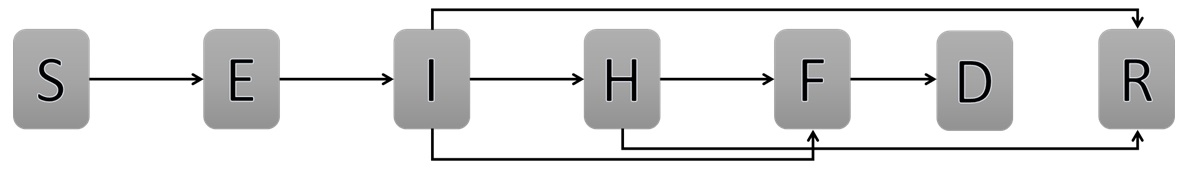
\includegraphics[width=1\textwidth]{compartmentNoFlow}
%  \caption{Compartment Model of the Ebola Epidemic in Liberia. \newline  Being S: Susceptible, E: Exposed, I: Infectious, H: Hospitalized, F: Funeral,  R: Recovered and D: Dead.  } 
%\label{fig:compartmentNoFlow} 
%\end{figure}

%\begin{description}
%\item[S]- Susceptible. Individuals who have not contracted the disease and have no immunity to it. 
%\item[E] - Exposed. Individuals who have come in contact with the Ebola patient and have contracted the disease but do not yet exhibit severe symptoms and thus, are considered not infectious.
%\item[I] - Infected. Individuals who experience severe symptoms of Ebola and are contagious.
%\item[H] - Hospitalized. Individuals who are infectious and are in the hospital because they are experiencing severe symptoms of Ebola.
%\item[F] - Funeral. Diseased but still contagious victims of Ebola. 
%\item[D] - Dead. Individuals who died because of Ebola and have been buried. They are considered not to be contagious.
%\item[R] - Recovered. Individuals who had Ebola, survived and now are immune to the disease.
%\end{description}


\subsection{Assumptions and Parameters}
We assume that no births or deaths occur during the modeled time period, other than the deaths related to Ebola. The relevant parameters are listed in Table \ref{tab:knownParameters} and Table \ref{tab:calibratedParameters}, with the latter calibrated for Liberia.
%\item We consider two time periods. The first one starts with the announcement of Ebola outbreak in March 2014 and ends the day of the International Intervention in September 2014. The second period covers the time from the International Intervention to July 2015.
%\end{itemize}

\begin{table}[ht]
\centering % used for centering table
\begin{tabular}{c c c}
\hline\hline %inserts double horizontal lines
Parameter & Value  & Reference \\ [0.5ex]
\hline % inserts single horizontal line
Incubation Period (${t_{P}}$) & 11 days & \cite{WHOFacts} \\
Duration of Traditional Funeral (${t_{F}}$) & 2 days & \cite{Rivers2014} \\
Time of Infection to Recovery (${t_{I}}$) & 10 days & \cite{Rivers2014} \\
Time from Infection to Death (${t_{D}}$) & 8 days & \cite{Rivers2014} \\
Case Fatality Rate, Unhospitalized ($\delta_{1}$) & 0.5 & \cite{WHOFacts} \\
Case Fatality Rate, Hospitalized ($\delta_{2}$) & 0.5 & \cite{WHOFacts} \\ [1ex]
\hline
\end{tabular}
\caption{Model Parameters for Ebola Epidemic in Liberia with literature citations.} % title of Table
\label{tab:knownParameters}
\end{table}

\clearpage